\documentclass{article}

\usepackage{graphicx}
\usepackage[serbianc]{babel}
\usepackage{multirow}
\usepackage{color}
\usepackage{amssymb}
\usepackage{colortbl}
\usepackage{multirow}
\usepackage[table]{xcolor}
\usepackage{array}
\usepackage{arydshln}
\usepackage{gensymb}
\usepackage{float}
\usepackage{url}
\usepackage[sorting=none]{biblatex}
\usepackage{color,soul}
\usepackage{caption}
\usepackage{amsmath}
\usepackage{pdfpages}

\usepackage[a4paper,
left=1in,
right=1in,
top=1in,
bottom=1in]{geometry}

\addbibresource{references.bib}
\definecolor{siva}{RGB}{0,34,85}

\definecolor{Gray}{gray}{0.8}
\newcolumntype{g}{>{\columncolor{Gray}}c}
\newcommand{\CellCol}[1]{\multicolumn{1}{>{\columncolor[gray]{.8}}c}{#1}}
\renewcommand{\listfigurename}{Списак слика}
\renewcommand{\listtablename}{Списак табела}
\renewcommand*\contentsname{Садржај}
\newcommand{\dd}[1]{\mathrm{d}#1}
\pagenumbering{gobble}

\begin{document}

\begin{center}
\begin{tabular}{ccc}
    {
\includegraphics[width=0.75in]{Images/UNS.jpeg}}
    & 
    \raisebox{0.3in}{
    \large
    \begin{tabular}{c}
        УНИВЕРЗИТЕТ У НОВОМ САДУ \\
        \textbf{ФАКУЛТЕТ ТЕХНИЧКИХ НАУКА}
        \\
        \textbf{У НОВОМ САДУ}
    \end{tabular}}
    &
    {
\includegraphics[width=0.75in]{Images/FTN.png}}
    \\
    \hline
\end{tabular}
\end{center}

\vspace{1in}
\begin{flushleft}
{\LARGE Срђан Апостоловић}
\end{flushleft}

\vspace{1.5in}
\begin{center}
    \textbf{\LARGE{Развој дела управљачког систeма \textit{Human Robot Collaborative} тропрсте роботске шаке}}
    \ \\
    \ \\
    \ \\
    \ \\
    \ \\
    \ \\
    {\LARGE ЗАВРШНИ РАД}
    \ \\
    \ \\
    \begin{tabular}{c}
         \hline\\

         {\Large Основне академске студије}
    \end{tabular}
\end{center}
\vspace{3.3in}
\begin{center}
Нови Сад, 2024.
\end{center}

\clearpage

\begin{center}
\begin{tabular}{|c|c|}
\hline
     & \ \\
    \multirow{3}{*}{{
\includegraphics[width=0.75in]{Images/FTN.png}}}
    & 
    УНИВЕРЗИТЕТ У НОВОМ САДУ  \textbf{ {\large$\cdot$} ФАКУЛТЕТ ТЕХНИЧКИХ НАУКА} \\
     & 21000 НОВИ САД, Трг Доситеја Обрадовића 6 \\
     \cline{2-2} & \cellcolor{gray!25}\ \\
     & \cellcolor{gray!25}КЉУЧНА ДОКУМЕНТАЦИЈСКА ИНФОРМАЦИЈА \\
     & \cellcolor{gray!25}\ \\
    \hline
\end{tabular}
\end{center}

\renewcommand{\arraystretch}{1.5}
\begin{tabular}{ll:lc}
\hline
\multicolumn{2}{l:}{Редни број, \textbf{РБР:}} & \\
\hdashline
\multicolumn{2}{l:}{Идентификациони број, \textbf{ИБР:}} & \\
\hdashline
\multicolumn{2}{l:}{Тип документа, \textbf{ТД:}} & \multicolumn{2}{l}{монографска документација}\\
\hdashline
\multicolumn{2}{l:}{Тип записа, \textbf{ТЗ:}} & \multicolumn{2}{l}{текстуални штампани материјал}\\
\hdashline
\multicolumn{2}{l:}{Врста рада, \textbf{ВР:}} & \multicolumn{2}{l}{завршни рад}\\
\hdashline
\multicolumn{2}{l:}{Аутор, \textbf{АУ:}} & \multicolumn{2}{l}{Срђан Апостоловић}\\
\hdashline
\multicolumn{2}{l:}{Ментор, \textbf{МН:}} & \multicolumn{2}{l}{проф. др Мирко Раковић}\\
\hdashline
\multicolumn{2}{l:}{Наслов Рада, \textbf{НР:}} & \multicolumn{2}{l}{
\begin{minipage}[t]{3.4in}
    Развој дела управљачког систeма \textit{Human Robot Collaborative} тропрсте роботске шаке
\end{minipage}}\\
\hdashline
\multicolumn{2}{l:}{Језик публикације, \textbf{ЈП:}} & \multicolumn{2}{l}{српски/ћирилица}\\
\hdashline
\multicolumn{2}{l:}{Језик извода, \textbf{ЈИ:}} & \multicolumn{2}{l}{српски}\\
\hdashline
\multicolumn{2}{l:}{Земља публиковања, \textbf{ЗП:}} & \multicolumn{2}{l}{Република Србија}\\
\hdashline
\multicolumn{2}{l:}{Уже географско подручје, \textbf{УГП:}} & \multicolumn{2}{l}{АП Војводина}\\
\hdashline
\multicolumn{2}{l:}{Година, \textbf{ГО:}} & \multicolumn{2}{l}{2024.}\\
\hdashline
\multicolumn{2}{l:}{Издавач, \textbf{ИЗ:}} & \multicolumn{2}{l}{ауторски репринт}\\
\hdashline
\multicolumn{2}{l:}{Место и адреса, \textbf{МА:}} & \multicolumn{2}{l}{
    \begin{minipage}[t]{3.5in}
        Нови Сад, Факултет техничких наука, Трг Доситеја Обрадовића 6
    \end{minipage}}\\
\hdashline
\multicolumn{2}{l:}{Физички опис рада, \textbf{ФО:}} & \multicolumn{2}{l}{12/41/11/5/17/0/0}\\
\hdashline
\multicolumn{2}{l:}{Научна област, \textbf{НО:}} & \multicolumn{2}{l}{мехатроника}\\
\hdashline
\multicolumn{2}{l:}{Научна дисциплина, \textbf{НД:}} & \multicolumn{2}{l}{роботика}\\
\hdashline
\multicolumn{2}{l:}{
    \begin{minipage}[t]{2.3in}
        Предмет одредница/Кључне речи, \textbf{ПО:}
    \end{minipage}} & робот, шака, ПЦБ\\
\hdashline
\multicolumn{2}{l:}{\textbf{УДК:}} & \\
\hdashline
\multicolumn{2}{l:}{Чува се, \textbf{ЧУ:}} & \multicolumn{2}{l}{
    \begin{minipage}[t]{3.5in}
        Библиотека Факултета техничких наука, Трг Доситеја Обрадовића 6, Нови Сад
    \end{minipage}}
    \\
\hdashline
\multicolumn{2}{l:}{Важна напомена, \textbf{ВН:}} & \\
\hdashline
\multicolumn{2}{l:}{Извод, \textbf{ИЗ:}} & \multicolumn{2}{l}{
  \begin{minipage}[t]{3.4in}
    Рад описује процес израде софтвера за управљање и комуникацију са роботскком шаком, 
    као и процес израде штампане плочице и њено програмирање у циљу остварења
    интерфејса рачунар-шака.
  \end{minipage}}
    \\
\hdashline
\multicolumn{2}{l:}{Датум прихватања теме, \textbf{ДП:}} & \\
\hdashline
\multicolumn{2}{l:}{Датум одбране, \textbf{ДО:}} & \\
\hdashline
Чланови комисије \textbf{KO}: & Председник: & Име презиме\\
\cdashline{2-4}\cline{4-4}
                              & Члан: & Име презиме & \multicolumn{1}{|c|}{Потпис ментора}\\
\cdashline{2-3}\cline{4-4}
                              & Члан, ментор: & др Мирко Раковић \hspace*{25mm}& \multicolumn{1}{|c|}{\ }\\
\hline

\end{tabular}

\clearpage

\begin{center}
    \begin{tabular}{|c|c|p{1in}|}
    \hline
        \multirow{4}{*}{{
\includegraphics[width=0.6in]{Images/FTN.png}}}
        & 
        УНИВЕРЗИТЕТ У НОВОМ САДУ  \textbf{ {\large$\cdot$} ФАКУЛТЕТ ТЕХНИЧКИХ} 
        & Број: \\
        \cline{3-3} & \textbf{НАУКА} & \ \\
        \cline{3-3} & 21000 НОВИ САД, Трг Доситеја Обрадовића 6 & Датум: \\
        \cline{2-3} & \cellcolor{gray!25}ЗАДАТАК ЗА ЗАВРШНИ РАД & \\
    \hline
    \end{tabular}
\end{center}

\begin{center}
    \begin{tabular}{|l|l|l|l|}
    \hline
        Студијски програм: & \multicolumn{3}{|l|}{Мехатроника} \\
        \hline Студнт: & Срђан Апостоловић \hspace{1.65in} & Број индекса: & MH6/2020 \\
        \hline Степен и врста студија: & \multicolumn{3}{|l|}{Основне академске студије} \\
        \hline Област: & \multicolumn{3}{|l|}{Мехатроника} \\
        \hline Ментор: & \multicolumn{3}{|l|}{проф. др Мирко Раковић} \\
        \hline \multicolumn{4}{|l|}{
            \begin{minipage}[t]{6.5in}
                НА ОСНОВУ ПОДНЕТЕ ПРИЈАВЕ, ПРИЛОЖЕНЕ ДОКУМЕНТАЦИЈЕ И ОДРЕДБИ СТАТУТА ФАКУЛТЕТА
                 ИЗДАЈЕ СЕ ЗАДАТАК ЗА ЗАВРШНИ РАД, СА СЛЕДЕЋИМ ЕЛЕМЕНТИМА:
                 \\
                -    проблем – тема рада;
                \\
                -    начин решавања проблема и начин практичне провере резултата рада, ако је таква проверанеопходна;
            \end{minipage}        
        }\\
        \hline
    \end{tabular}
\end{center}
\ \\
\ \\
\large \textbf{НАСЛОВ ЗАВРШНОГ РАДА:}
\ \\
\fbox{Развој дела управљачког систeма \textit{Human Robot Collaborative} тропрсте роботске шаке \hspace{5mm}}
\ \\
\ \\
\large \textbf{ТЕКСТ ЗАДАТКА:}
\ \\
\begin{tabular}{|p{6.5in}|}
    \hline
        Осмислити, пројектовати и дизајнирати софтвер за управљање роботском шаком и штампану плочицу која представља хардверски интерфејс шака-рачунар. \\
    \hline
\end{tabular}
\ \\
\begin{center}
    \begin{tabular}{|p{3.16in}|p{3.16in}|}
    \hline
        Руководилац студијског програма: & Менотр рада:\\
        \hline проф. др Мирко Раковић & проф. др. Мирко Раковић\\
        \hline
    \end{tabular}
\end{center}
\ \\
\begin{center}
    \begin{tabular}{|p{6.5in}|}
    \hline
        Примерак за: \makebox[4mm][l]{$\square$} - Студента; \makebox[4mm][l]{$\square$} - Ментора \\
    \hline
    \end{tabular}
\end{center}

\clearpage
\tableofcontents
\clearpage
\pagenumbering{arabic}
\clearpage
\listoffigures
\clearpage
\listoftables
\clearpage


\section{Увод}
У свету роботике, који свакодневно напредује, заједно са самим роботима напредују
и алати које роботи користе. Како је један од главних задатака робота да ухвати предмет рада и 
њиме даље манипулише, настала је потреба и за хватаљкама које омогућавају обављање таквих
типова задатака. \\Постоје различите имплементације роботских хватаљки, међу које спадају
и роботске шаке. Главна подела роботских шака се заснива на броју прстију, и постоје три 
велике групе : двопрсте, тропрсте и петопрсте шаке. Као што им име и само говори 
двопрсте шаке имају два, тропрсте три, а петопрсте пет прстију. У зависности од имплементаицје, 
прсима је могуће управљати заједно или одвојено, односно независно једно од других. Даља подела се заснива на броју 
степени слободе у прстима. \hl{Сваки прст може да бити фиксан или да се помера у односу на корен шаке 
само по једној оси. Такође прст може имати више мотора који га контролишу чиме може да оствари мноштво различитих положаја}. 
Роботска шака са три прста предтавља компромисно решење између 
двопрсте и петопрсте шаке.\\
\hl{У односу на двопрсту шаку, тропрста има могућност оставаривања већег броја различитих
хватова. (* mislim da svaka troprsta saka moze da ostavari vise razlicitih hvatova od dvoprste jer je uvek barem jedan 
prst slobodan da se krece po tri ose, sto znatno dodaje na razlicitosti hvatova *) Својом конструкцијом, тропрста шака остварује могућност да се прилагођава предметима разних облика и величина.} У поређењу
са петопрстом шаком, тропрста јесте генерално лошија. Као резултат те разлике, тропрст шака је јефтинија, што у мање захтевним 
задацима 
не преставља проблем и представља компромисно решење као алат који ће се корстити на индустријском роботу.\\
\indent Шака која је тема овог рада, \textit{Human-Robot Collaborative
(HRC) Hand} је тропрста шака. Конструкција \textit{HRC} шаке омогућава да се два прста крећу у оквиру 
својих засебних равни, то јест да врше флексију и екстензију, као што је приказано на слци 1.а. Трећи прст, палац, има слободу кретања у 
тродимензионалном простору у односу на корен шаке, односно додатно може да врши адукцију и абдукцију, као што је 
приказано на слици 1.б. Важно је напоменути да су 
прсти \textit{HRC} шаке подактуисани, односно да само један мотор погони цео прст.
\begin{figure}[H]
\centering
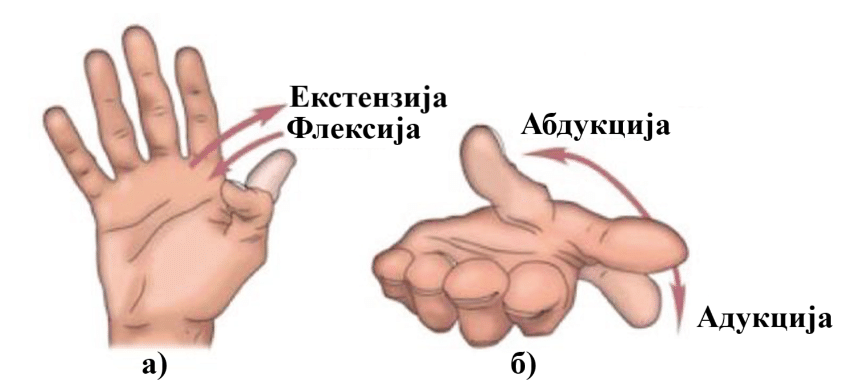
\includegraphics[height=2in]{Images/Slika1.png}
\caption{Померање прстију људске шаке. \\ а) флексија и рефлексија, б) адукција и абдукција \cite{abduction}}
\label{fig:figure1}
\end{figure}
\subsection{Методологија рада}
Рад који следи има за циљ да покаже један од могућих приступа решавању проблема 
управљања положајем, брзином и убрзањем мотора једносмерне струје. Такође рад покзајуе 
приступ имплементацији комуникације између
управљачке електронике мотра и корисничког рачунанра, у сврху покретања роботског 
манипулатора, односно роботске шаке. \\
\ \\
\hl{Механичка конструкција \textit{HRC} шаке као и 
управљачка електроника за покретање мотора дизајнирани су 
од стране факултета. На основу постојеће управљачке електронике, било је потребно развити програмско решење 
за управљање шаком, као и наменску електронику за комуникацију шаке са персоналним рачунаром.
Зарад остваривања комуникације између роботске шаке и корисничког рачунанра, као и обезбеђивање
напајања управљачке електронике мотора било је
потребно произвести интерфејс. Циљ оваквог интерфејса је да на што лакши
начин омогућити кориснику комуникацију са роботском шаком. Такође развијена је и 
програмска библиотека, помоћу које се команде са рачунара шаљу ка управљачкој електроници.}\\
Етапе по којима су решавани задаци овог дипломског рада су:
\begin{itemize}
    \item Развој управљачког алгоритма за моторе прстију шаке
    \item Дизајнирање \textit{НCU} штампане плочице 
    \item Развој програма за \textit{Hand Control Unit (HCU)} штампану плочицу
    \item Развој програмске библиотеке за виши ниво управљања шаком
\end{itemize}
\ \\
\clearpage
\section{Преглед стања}
На тржишту постоје разна техничка решења роботиских шака. У даљем тексту ће
бити дат преглед четири популарне роботске шаке, а то су : 
\begin{itemize}
    \item \textit{Shadow DEX-EE} \cite{shadow_rob}
    \item \textit{Robotiq 3-finger adaptive gripper} \cite{robotique}
    \item \textit{BarrettHand} \cite{barret}
    \item \textit{Scramp’s multi-joint 3 finger Gripper} \cite{scram}
\end{itemize}
\subsection{\textit{Shadow DEX-EE}}
\textit{Shadow DEX-EE} је водећи производ настао сарадњом компаније \textit{Shadow Robot} и 
\textit{Google DeepMind}. Циљ ове сарадње, односно роботске шаке је да омогући што лакши 
начин интеграције принципа машинског учења у реаланoм свету роботике и технике. Приказ \textit{Shadow DEX-EE} роботске
шаке дат је на слици 2.\\
Прсте ове роботске шаке погони пет мотора. Три мотора су задужена за флексију и екстензију подактуисаних прстију, док друга два мотора 
врше адукцију и абдукцију два прста. \\
Шака у средини длана садржи стерео камеру која шаље информацију о положају шаке у односу на предмет манипулисања роботу.
Овако добијена информација омогућава додатну прецизност приликом хватања предмета. Комуникација
између корисничког рачунара и шаке се остварује путем \textit{EtherCAT} комуникационог протокола.\\ 
Управљање самим моторима шаке је заснована на \textit{Proportional Integral Derivative(PID)} \cite{pid} регулатору, 
и имплементирана су три контролера у каскадној вези. Струјна петља каскадне везе регулатора се извршава са фреквенцијом 
од 5 kHz, док се петље брзине и позиције извршавају са учестаношћу од 1 kHz.\\
Максмиална сила коју \textit{Shadow DEX-EE} остварује је 8 N на врху прста, док је брзина померања прста 180 \degree/s.
На врху сваког прста се налази сензор силе, чиме ова шака има могућност прилагођавања силе стиска, 
као и самог хвата у односу на објекат манипулације. Максимална носивност шаке износи 3 kg. \cite{shadow_rob}
\begin{figure}[H]
\centering
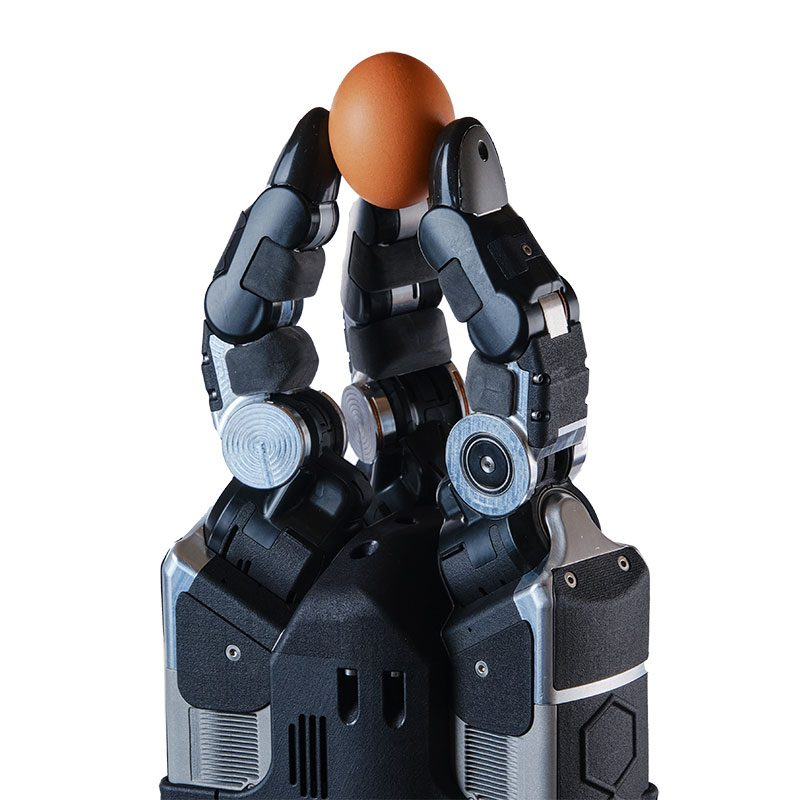
\includegraphics[width=2in, height=2in]{Images/Saka1.jpg}
\caption{Роботска шака \textit{Shadow DEX-EE}. \cite{shadow_rob}}
\label{fig:figure2}
\end{figure}
\subsection{\textit{Robotiq 3-finger adaptive gripper}} 
\textit{Robotiq 3-finger adaptive gripper}, приказан на слици 3, представља роботску шаку дизајнирану за употребу 
у индустрији као алат на роботској руци. \hl{Како је ово индустријски производ, велики број података произвођач 
није поставио доступним.\\ 
Палац ове шаке има могућност кретања у једној равни, док 
преостала два прста поседују могућност независног кретања у тродимензионалном простору.}\\
Шака подржава мноштво индустријских комуникационих протокола као што су 
\textit{Modbus TCP, PROFINET, EtherCAT, CANopen}.\\
Прецизност позиционирања врха пртију износи 0.05 mm. Максимална сила стиска шаке је 80 N, док је минимална 30 N. 
Максимална носивост износи 10 kg, док је максималан хват шаке 155 mm. \cite{robotique}
\begin{figure}[H]
\centering
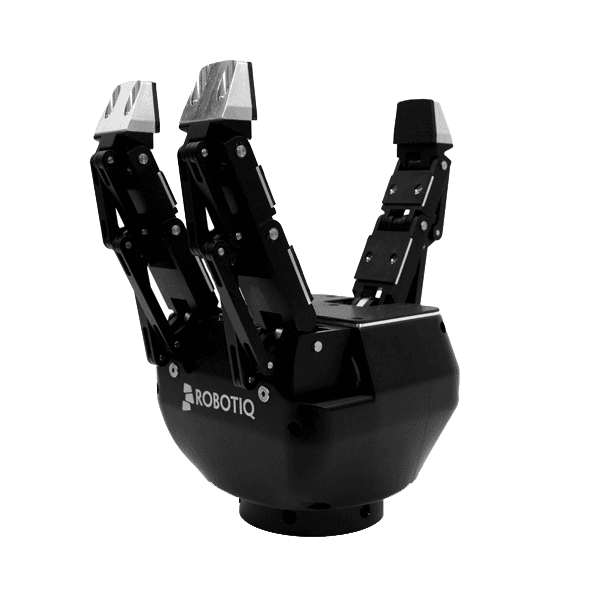
\includegraphics[width=3in, height=3in]{Images/Saka2.png}
\caption{Роботска шака \textit{Robotiq 3-finger adaptive gripper}. \cite{robotique}}
\label{fig:figure3}
\end{figure}
\subsection{\textit{BarrettHand}} 
\textit{BarrettHand}, приказана на слици 4, је још једна роботска шака првенствено дизајнирана за експлоатацију у индустрији. 
Слично као и \textit{Robotiq gripper}, палац се креће по две осе, док друга два прста засебно могу да
се крећу по три осе. \\Како је шака дизајнирана
за рад у условима где је електро-магнетни шум реалан проблем, комуникација између рачунара и шаке cе одвија путем \textit{Controller Area Network (CAN)} \cite{can}
комуникационог протокола. \\
Максмимална брзина затварања прстију износи 360 \degree/s, док је максимална носивност 6 kg. \\
Мерни уређај за одређивање позиције прстију је Холов сензор (енг. \textit{Hall sensor}). Пренос момента, односно силе од вратила мотора ка 
врховима прстију је реализован користећи пужне зупчасте парове. На врховима прстију се налазе сензори силе чиме се постиже 
могућност прилагођавања хватања предмета. Максималан хват шаке износи 335 mm. \cite{barret}
\begin{figure}[H]
\centering
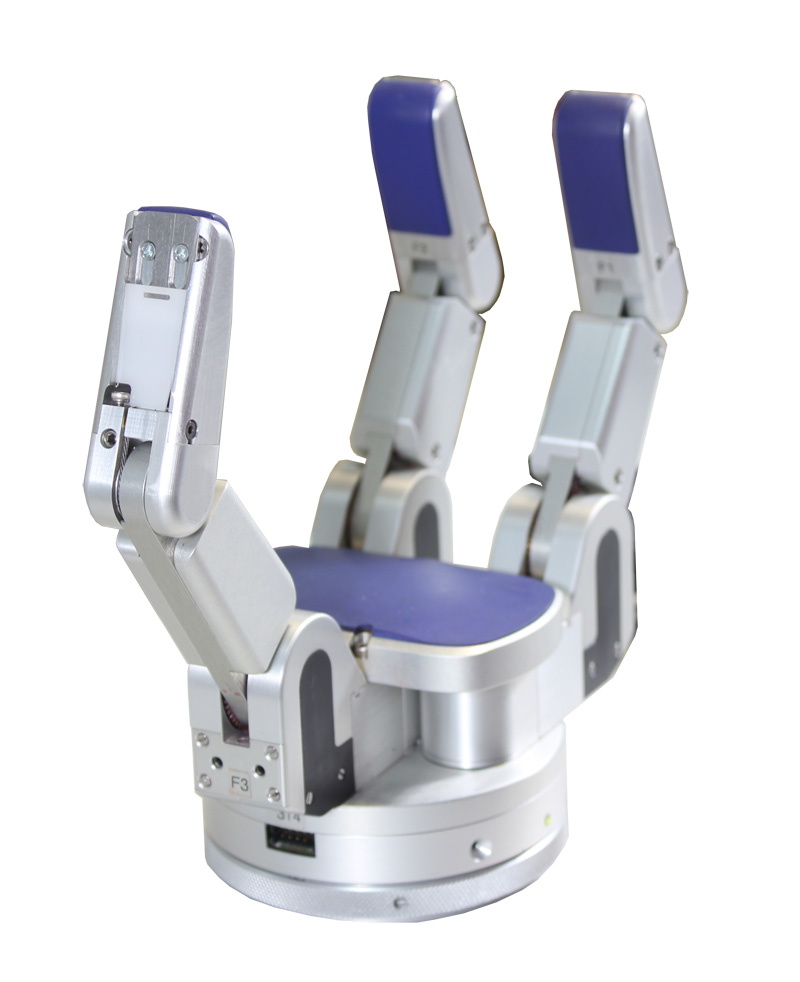
\includegraphics[width=3in, height=3in]{Images/Saka3.jpg}
\caption{Роботска шака \textit{BarrettHand}. \cite{barret}}
\label{fig:figure4}
\end{figure}
\subsection{\textit{Scramp’s multi-joint 3 finger Gripper}} 
\textit{Scramp’s multi-joint 3 finger Gripper}, \hl{приказан на слици 5, представља механички најкомплексније решење тропрсте шаке зато што омогућава засебно 
управљање са сва три прста по све три просторне осе.} \\Mаксмиална брзина затварања прстију износи 210 \degree/s. Као и претходне роботске шаке, и 
\textit{Scramp’s multi-joint 3 finger Gripper} садржи сензоре силе на врховима прстију.\\Комуникација између рачунара и шаке је, као и код \textit{BarrettHand} реализована 
путем \textit{CAN} комуникационог протокола.  \cite{scram}
\begin{figure}[H]
\centering
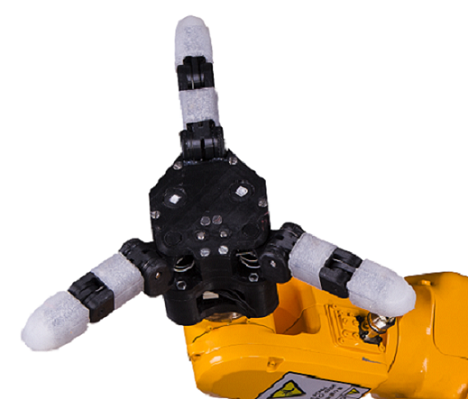
\includegraphics[width=3in, height=3in]{Images/Saka4.png}
\caption{Роботска шака \textit{Scramp’s multi-joint 3 finger Gripper}. \cite{scram}}
\label{fig:figure5}
\end{figure}
\clearpage

\section{Механички склоп \textit{Human-Robot Collaborative} шаке}
\textit{Human-Robot Collaborative} роботска шака, приказана на слици 6, је тропрста роботска шака и тиме
механички склоп можемо поделити у четири целине.\\ 
Основа шаке, односно база преставља централни део који у себи
носи две \textit{Finger Control Unit (FCU)} штампане плочице. \textit{FCU} штампане плочице представљају управљачку електронику за по два 
Мaxon DCX22L мотора једносмерне струје. Такође у бази шаке се налази и \textit{Hand Control Unit (HRC)} штампана плочица која представља интерфејс 
рачунар - шака. Шака на свом кућишту има четири конекотра која служе за напајање и програмирање електронике
унутар саме шаке како би се развој и рад са њом у што већој мери упростио крајњем кориснику.\\

\begin{figure}[H]
\centering
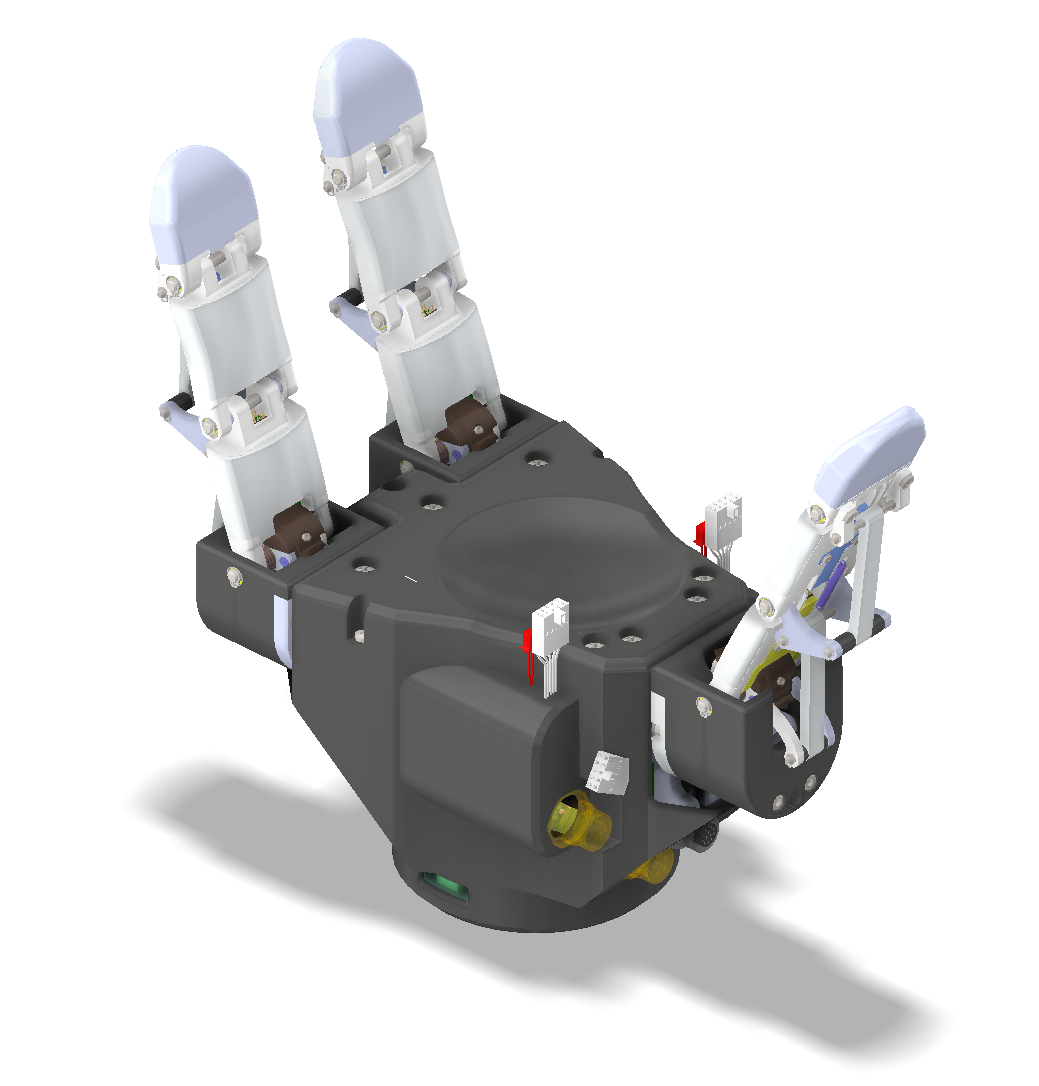
\includegraphics[width=3in, height=3in]{Images/Saka.png}
\caption{Приказ тродимензионалног модела \textit{HRC} шаке.}
\label{fig:figure6}
\end{figure}
\ \\
Кућиште и три прста су израђена методом селективног ласерског синтеровања пластике (енг. \textit{Selective laser sintering (SLS)}).
Као резултат добијено је чврсто кућиште, комплексне геометрије које штити електронику и моторе од спољашњих утицаја, прљавштине и 
случајних механичких оштећења током рада.\\
\ \\
Поред базе, шака поседује и три прста. Два прста су погоњена са по једним мотором, чиме остварују слободу кретања по две осе,
док је трећи прст, односно палац, погоњен са два мотора и тиме поред кретања сличном преостала два прста, има могућност
ротирања и око треће осе.\\
На врху сваког прста се налази сензор силе \textit{Force Sense Unit (FSU)}, који даје информацију о тренутној сили стиска
на основу које се даље управља радом шаке. Сигнал се од \textit{FSU} сензора до \textit{FCU} штампане плочице преноси путем 
клизних прстена (енг. \textit{slip ring}) чиме се потреба за повезивањем жицама избацује. Резултат
је смањена могућност настнка проблема приликом размене информација.\\
Прсти шаке су сачињени од по три сегмента. Важно је напоменути да је специфичност ове роботске шаке чињеница да су прсти подактуисани, 
односно да мотор гони само сегмент прста најближи бази шаке, док се померање осталих чланова прстију врши преко система полуга и опруга. 
Погонски момент се од мотора, до првог сегмента прста преноси путем зупчастих
парова, што омогућава да се оса ротације мотора измести у односу на осу ротације прста, и добије компактније механичко 
решење. Зупчаници су израђени од бронзе и челика, те је механичко хабање током рада минимално.

\clearpage

\section{Електрични систем \textit{Human-Robot Collaborative} шаке}

Како би се омогућило покретање мотора, односно прстију, било је потребно пројектовати две различите штампаме плочице. 
\textit{Finger Control Unit} штампана плочица је пројектована од стране професора са катедре 
у сарадњи са компанијеом \textit{HTEC GROUP DOO}. Задатак ове плочице је да, на основу информација које добије 
путем \textit{CAN} комуникационог протокола од стране \textit{Hand Control Unit} штампане плочице, 
покрене моторе на одговарајућ начин.\\ 
\textit{Hand Control Unit} штампана плочица је била један од задатака овог дипломског рада. 
Један од њених задатака је био да сигнал примљен од стране рачунара путем \textit{Universal Serial Bus (USB)} комуникационог 
протокола обради и проследи на одговарајући \textit{FCU}. Поред комуникације, \textit{НCU} има за задатак да улазно напајање 
од 24 V спусти на 18 V, а да при томе омогући континуалан проток струје од 5 А за сваки \textit{FCU}.
\begin{figure}[H]
\centering
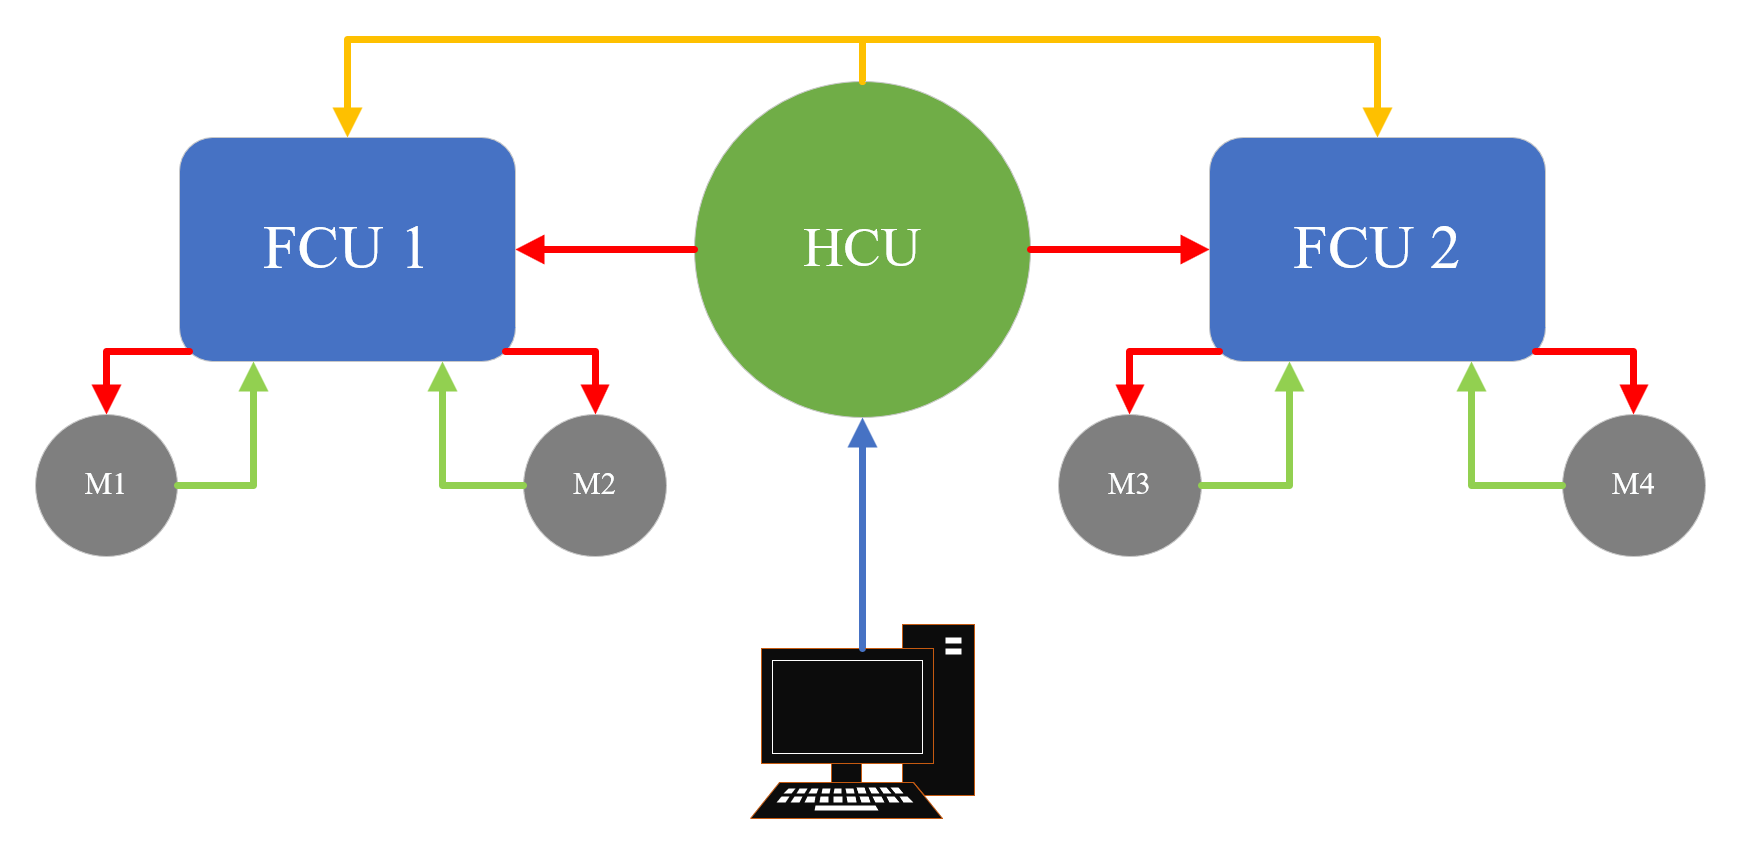
\includegraphics[height=2in]{Images/SemaElektronika.png}
\caption{Шематски приказ повезивања електрноике \textit{HRC} шаке.}
\label{fig:figure7}
\end{figure}
\subsection{\textit{Hand Control Unit} штампана плочица} 
\textit{Hand Control Unit} штампана плочица (Слика 10.) је хадрверски интерфејс између рачунара и \textit{FCU} плочица. Њен задатак је да команду
за обртање мотора, добијену са рачунара преусмери ка \textit{FCU} плочицама. Приликом обраде команде са рачунара, потребно је претворити
\textit{USB} поруку у \textit{UART} поруку како би микроконтролер знао да је обради. Након дојене \textit{UART} поруке, потребно је 
проследити жељену команду у виду \textit{CAN} поруке. Поред комуникације, \textit{HCU} штампана плочица треба да улазно напајање у систем 
од 24 V, спусти на три различита напонска нивоа. Први нивоје је 3,3 V са којима се напаја сам микроконтролер. Други напонски ниво је 
5 V коришћен за напајање интегрисаних кола за претварање комуникационих сигнала. Последњи напонски ниво је 18 V којим се напајају \textit{FCU}
штампане плочице. Поред претварања напона на 18 V, додатан проблем је био и омогућавање константе струје од 5 А, која је потребна за управљање 
моторима. Компоненте које су коришћене за постизање жељених функионалности су : \\
\begin{itemize}
    \item \textit{STM32L432KC} микроконтролер \cite{stm32_l4_data} \cite{stm32_l4_ref} \cite{stm32_l4_prog}
    \item \textit{MCP2551 CAN} трансивер  \cite{mcp2551}
    \item \textit{CH340C USB} на \textit{UART} конвертер \cite{ch340c}
    \item \textit{SIC437AED} спуштач напона (енг. \textit{buck converter}) \cite{vishay}
    \item \textit{AP63203 и AP63205} спуштачи напона \cite{ap6320}
\end{itemize}

\begin{figure}[H]
\centering
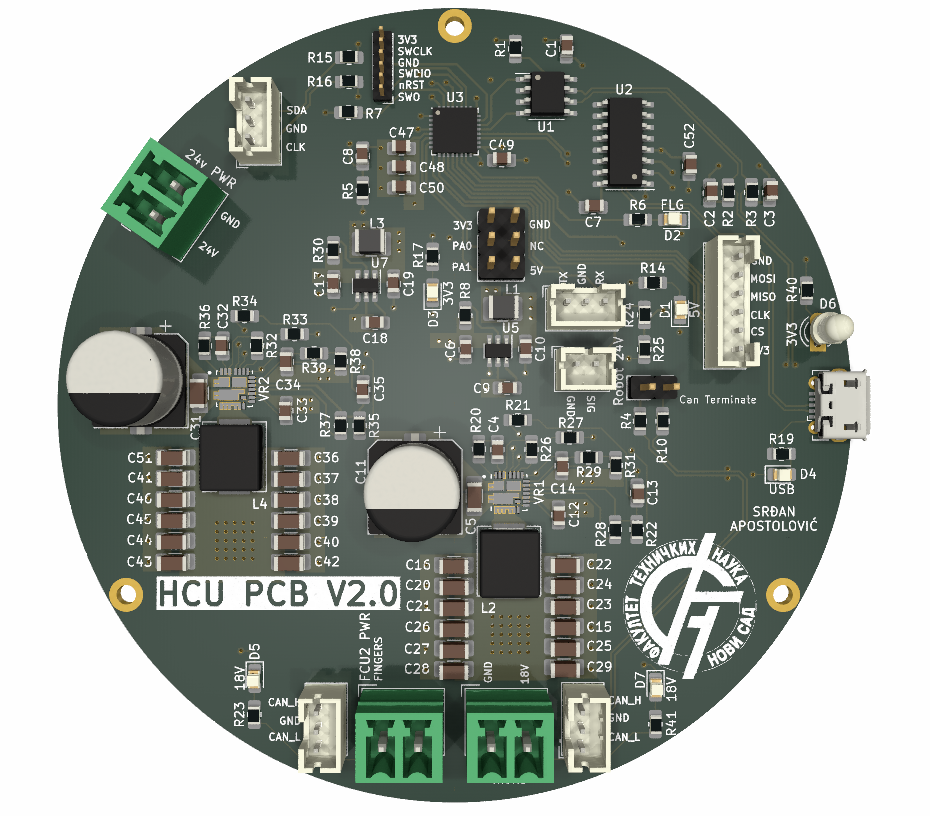
\includegraphics[height=3in]{Images/HCU.png}
\caption{\textit{Hand Control Unit} штампана плочица}
\label{fig:figure8}
\end{figure}

\subsubsection{\textit{STM32L432KC} микроконтролер} 
\textit{STM32L432KC} микроконтролер је микроконтролер компаније \textit{ST Microcontrollers} са максимално фреквенцијом радног клока од 80 MHz.
Захтеви за димензијама \textit{HCU} штампане плочице су наметале ограничења при избору компоненти, и тиме је овај микроконтролер 
изабран као решење. Поред малих карактеристика, овај микроконтролер има имплементирано мноштво комуникационих протокола, што 
доказује и чињеница да се може наћи и у уређајима за рачунаре као што су тастатуре. Комуникациони протоколи који су имплементирани на 
овом микроконтролеру као део овог дипломско рада су \textit{CAN} и \textit{UART}.

\subsubsection{\textit{MCP2551 CAN} трансивер} 
\textit{MCP2551 CAN} трансивер је најпознатије \textit{CAN} трансивер интегрисано коло на свету, и може се наћи у мноштву \textit{CAN}
експанзионих плочица и модула на тржишту. Због распрострањености и коришћености овог интегрисаног кола, могуће је наћи веома пуно примера коришћена 
овог кола у електричним уређајима и шемама, чиме је процес дизајнирања \textit{HCU} штампане плочице упрошћен, али је вероватноћа добијања 
уређаја који ради знатно повећана. Као резултат овог приступа решавању проблема \textit{CAN} комуникације добијено је веома 
компактно и просто решење које ради и успешно остварује комуникацију између \textit{HCU} и \textit{FCU} штампаних плочица.

\subsubsection{\textit{CH340C USB} на \textit{UART} конвертер} 
\textit{CH340C} интегрисано коло је коришћено да прилагоди информације добијене са рачунара микроконтролеру. 
Како се поруке од рачунара до \textit{HCU} штампане плочице преносе путем \textit{USB} комуникационог 
протокола, потребно их је претворити у \textit{UART} поруке. Ово интегрисано коло је изабрано због 
доступности, ниске цене и чињенице да му није потребан спољашњи осцилатор за генерисање такта.

\subsubsection{\textit{SIC437AED} спуштач напона}
\textit{SIC437AED} спуштач напона je синхрони спуштач напона са уграђеним \textit{MOSFET} \cite{mosfet} прекидачима 
за високи и ниски напонски ниво. Ово интегрисано коло омогућава континуалну струју од 12 А и фреквенцију прекидања 
излазног напона од маскимално 1 MHz. Улазни напон мора бити из опсега од 3 V до 28 V, док излазни напон може варирати 
између  0.6 V и маскмиалног улазног напона.\\
\textit{SIC437AED} имплементира пренапонску заштиту, заштиту од превелике излазне струје, заштиту од 
кратког споја као и заштиту од прегревања. Ово интегрисано коло такође поседује и програмабилни режим
постепеног укључења (енг. \textit{soft start}) како би се смањили струјни удари приликом стартовања система.\\
\textit{HCU} штампана плочица имплементира овај чип са циљем спуштања напона са 24 V на 
18 V, излазном фреквенцијом од 750 kHz и постепеним укључењем од 6 ms.

\subsubsection{\textit{AP63203 и AP63205} спуштачи напона}
\textit{AP63203 и AP63205} спуштачи напона напона су такође синхрони спуштачи напона са уграђеним \textit{MOSFET} прекидачима. Највећа предност коришћења ових 
интегрисаних кола је што обезбеђују сузбијање електромагнетног шума. Оба два интегрисана кола могу да омогуће максимлану континуалну излазну струју од 2 А и излазну фреквенцију прекидања од 1,1 MHz. За разлику од \textit{SIC437AED}, оба ова интегрисана кола имају фиксан излазан напон.
Разлика између \textit{AP63203} и \textit{AP63205} спуштача напона је излазни напон. Излазни напон \textit{AP63203} је 3 V, док је излазни напон \textit{AP63205} 5 V. Улазни напон \textit{AP63203} износи 
3.8 V, док улазни напон \textit{AP63205} износи 5,8 V.

\begin{figure}[H]
\centering
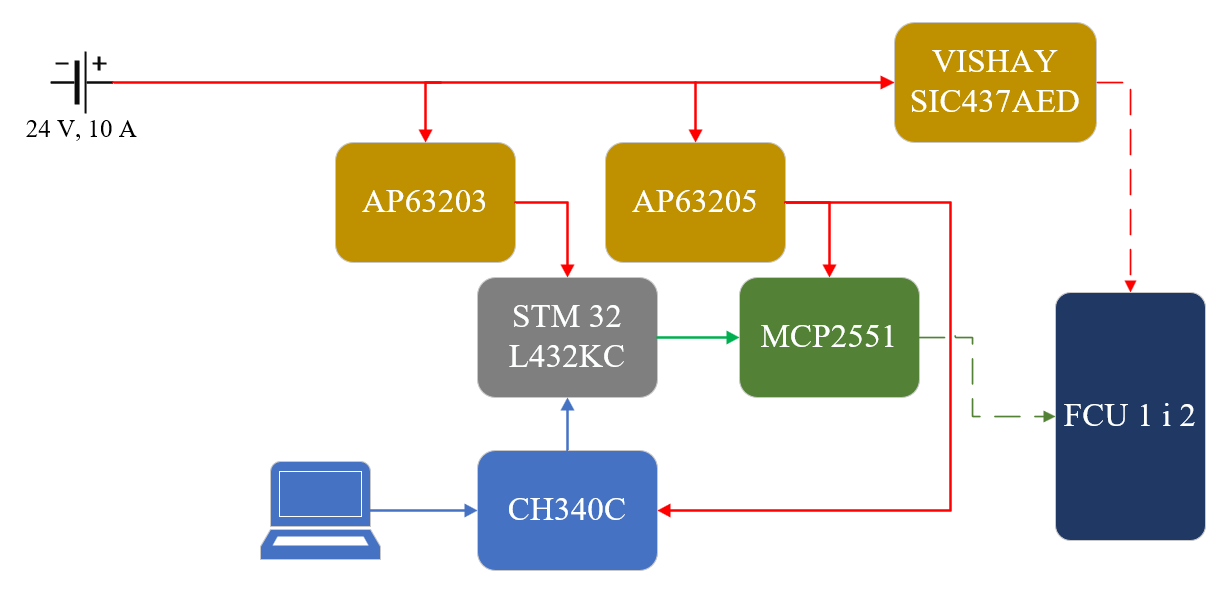
\includegraphics[height=3in]{Images/HCU_blok_sema.png}
\caption{Блок дијаграм \textit{Hand Control Unit} штампане плочице.}
\label{fig:figure9}
\end{figure}

\subsection{\textit{Finger Control Unit} штампана плочица} 
\textit{Finger Control Unit} штампана плочица, приказана на слици 9, представља управљачку електронику за два мотора једносмерне струје.\\ 
Команде о покретању мотора се добијају путем \textit{CAN} комуникационог протокола, од стране \textit{HCU} штампане плочице. Добијени подаци 
се прилагођавају користећи \textit{TCAN330 CAN} трансивер, и шаљу микроконтролеру на даљу обраду. Микроконтолер на основу добијених команди 
генерише \textit{Pulse Width Modulation (PWM)} сигнал којим управља \textit{MP6519} Х мостом. Х мост путем добијеног сигнала управља мотором, 
регулисањем струје на његовим прикључцима. Информације о положају и брзини обртања мотора, добијене од инкременталног енкодера, се кроз 
\textit{AM26LS32AC} интегрисано коло шаљу микроконтролеру. Поред управљана мотором, микроконтролер треба да путем \textit{SPI} комуникационог 
протокола информације од \textit{FSU} сензора силе проследи назад \textit{HCU} штампаној плочици.
\textit{FCU} плочица на себи 
садржи мноштво компонената како би остваривала свој задатак. У даљем тексту ће се обрадити само оне најважније, а то су :
\begin{itemize}
    \item \textit{STM32F405VGT6} микроконтролер \cite{stm32_f4_data}
    \item \textit{MP6519} Х моста са интегрисаним регулатором струје \cite{mp6519}
    \item \textit{TCAN330 CAN} трансивер \cite{tcan330}
    \item \textit{AM26LS32AC} интегрисано коло за обраду енкодерских сигнала \cite{am26ls32}
\end{itemize}


\begin{figure}[H]
\centering
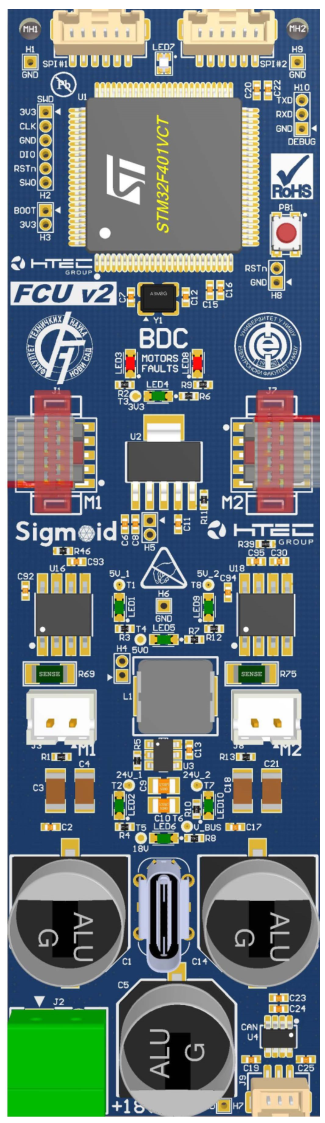
\includegraphics[height=2in]{Images/FCU.png}
\caption{\textit{Finger Control Unit} штампана плочица.}
\label{fig:figure10}
\end{figure}

\subsubsection{\textit{STM32F405VGT6} микроконтролер} 
\textit{STM32F405VGT6} микроконтролер преставља микроконтролер серије четири компаније \textit{ST Microelectronics}. Од значајних 
периферија контролер садржи бројачку, односно тајмер периферију са пет тајмера, \textit{CAN} периферију, \textit{General-purpose input/output (GPIO)} периферију и 
\textit{Serial Peripheral Interface (SPI)} \cite{spi} периферију.\\
Бројачи односно тајмери су подељени у три групе. Прва група су два тајмера код којих фактор испуне излазног \textit{Pulse width modulation (PWM)}
сигнала преставља жељену струју на улазу у мотор. Друга група су такође два бројача који служе да броје инкременте енкодера уз 
примену квадратурне модификације сигнала, чиме се даље одређује положај мотора. Пети, преостали тајмер се користи за генерисање 
софтверске прекидне рутине. У прекидној рутини петог тајмера се врши PID калкулација, одређивање положаја и брзине мотора као и синтеза брзине у 
зависности од пређеног пута, о чему ће бити речи касније у раду.\\
\textit{CAN} периферија микроконтролера служи за комуникацију са \textit{НCU} штампаном плочицом. \textit{CAN} комуникациони 
протокол представља идеално решења за услове рада у средини у којој има пуно електромагнетног шума, као што је непосредна околина
мотора једносмерне струје. Предност \textit{CAN} сигнала у односу на друге коминкационе сигнале је коришћење диференцијалног пара 
проводника кроз које се сигнал простире чиме се појава шума након трансиверског кола одстрањује.\\
\textit{GPIO} периферија је заслужна за управљање свом електроником која окружује микроконтролер. Конкретно на примеру ове плочице се
путем ове периферије улазни сигнали од енкодера, \textit{CAN} сингали и улазни \textit{SPI} сигнали преусмеравају ка одређеним 
интерним модулима микроконтролера, док се излазни сигнали попут укључивања прекидача за напајање, укључивање \textit{Light emmiting (LE)}
диода и \textit{PWM} сигнали воде ка одговарајућим извршним органима. \\
\textit{(SPI)} периферија служи за остваривање комуникације између \textit{FCU} и \textit{FSU} плочица. Имајући на уму да 
један \textit{FCU} контролише два мотора било је потрбно да микроконтролер саржи барем две \textit{(SPI)} периферије. \cite{stm32_f4_prog} \cite{stm32_f4_ref}

\subsubsection{\textit{MP6519} Х мост са регулатором струје}
\textit{MP6519} је интегрисано коло чији је задатак да на основу улаза даје одговарајућу струју на прикључцима мотора. Да би се 
тражена струја обезбедила интегрисано коло управља напоном на излазу. Коло у 
себи садржи регулатор струје, и на основу улазног \textit{PWM} сигнала, одређује излазну струју пропорционалну времену укључења
\textit{PWM} сигнала у току једног периода. Поред одређивања струје, коло садржи и једну ножицу помоћу које се одређује смер
обртања мотора. Такође је могуће контролисати излазну фреквенцију сигнала за управљање струјом. Како je временска константа 
коришћених мотора веома мала, фреквенција је подешена на 225 kHz чиме се смањује осциловање струје на прикључцима мотора.

\subsubsection{\textit{TCAN330 CAN} трансивер}
\textit{TCAN330 CAN} трансивер је интегрисано коло чији је задатак да \textit{CAN} сигнал са излаза микроконтролера, претвори 
у диференцијални пар сигнала, односно сигнале \textit{CAN HIGH} и \textit{CAN LOW}. Важно је напоменути да сигнал од микроконтролера 
до трансивер чипа има одвојене линије за слање и пријем порука, док после трансивера и ка \textit{НCU} штампаној плочици, пријем и 
слање порука се одвија на истој физичкој линији.

\subsubsection{\textit{AM26LS32AC} интегрисано коло за обраду енкодерских сигнала}
\textit{AM26LS32AC} интегрисано коло служи за обраду диференцијалних сигнала са енкодера мотора. Због велике
количине елктро-магнетног зрачења у околини мотора, сигнали А, Б и И се од енкодера мотора до \textit{FCU} 
штампане плочице преносе у виду диференцијалног пара. У случају настанка шума, диференцијални пар, након 
стастављана сигнала, одстрањује шум и обезбеђује тачну информацију за даљу обраду у циљу добијања информација 
о брзини и положају.

\subsection{\textit{Мaxon DCX22L} мотор једносмерне струје} 
Мaxon DCX22L (Слика 8.) мотори који су коришћени су мотори једносмерне струје, номиналног напона 18 V и номиналне струје 2.26 А. Номинална
брзина обртања вратила мотора износи 11800 обртаја у минути, док номиналан момент на излазу мотора износи 33 mNm. Номинална
брзина самог мотора је превелика за употребу у прецизном позиционирању, док је номиналан момент недовољан за задатке хватања предмета.
Проблеми превелике брзине и премалог момента су решени тростепеним редуктором на изалазу мотора са пренесним односом 172:1.
Губици који настају у редуктору не прелазе 10 посто што је задовољавајуће, а за коначну изалазну брзину добијамо 68,6 обртаја 
у минути, а излазни момент након редуктора износи 5,67 Nm. Поред реуктора мотор на другом крају садржи инкрементални енкодер који 
генерише 1024 импулса по кругу. Прецизност позиционирања вратила редуктора мотора, са оваквим уграђеним енкодером и применом 
квадратурне модификације сигнала износи 0.00051 \degree.\\
\begin{figure}[H]
\centering
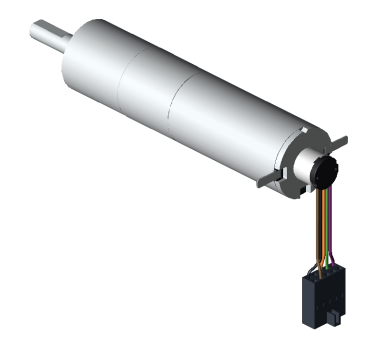
\includegraphics[height=2in]{Images/Maxon.png}
\caption{\textit{Мaxon DCX22L} мотор.}
\label{fig:figure11}
\end{figure}
\clearpage

\section{Тероијске основе рада}
У овом поглављу је дат преглед принципа рада коришћених технологија и метода. 
\subsection{Принцип рада мотора једносмерне струје са четкицама и сталчним магнетима}
Мотор једносмерне струје са четкицама \textit{(BDC motor)} је најчешће коришћен електро мотор. Свуда око нас се могу наћи различити мотори једносмерне струје
са четкицама, а неки од примера су : играчке аутомобила, брисачи на ауту, вентилатори у рачунару, акумулаторски алат и други. 
Конструкција \textit{HRC} шаке користи моторе једносмерне струје са четкицама и сталним магнетима.\ \\ \\ 
Мотор једносмерне струје је сачињен од две главне целине, ротор и статор. Ротор је сачињен од вратила мотора која се приликом довођења напона обрће, арматуре и намотаја проводника који се спаја са ламелама комутатора. Арматура је конструктивни део који служи као основа око које су намотани намотаји. Сачињена је од мноштва челичних лимова како би се утицај индукованих вртложних струја смањио. У зависности од конструкције ротор може садржати и више од једног сета намотаја проводника. Ламеле комутатора су у сталном контакту са графитним четкицама по којима се обрћу. Четкице мотора, су са друге стране спојене на спољашње прикључке мотора кроз које се доводи управљачки сигнал. Статор мотора је сачињен од кућишта и сталних магнета. Кућиште је произведено спајањем плочица од лима, слично као и код ротра, како би се у што већој мери смањио утицај вртложних струја. У тако израђено кућиште су утиснути магнети на тај начин да су полови два суседна магнета обрнуто оријентисани у односу један са другим. Северни магнетни пол једног магнета је окренут ка вратилу мотора, док је северни магнетни пол другог магнета окренут насупрот вратилу мотора. \\
Када се на прикључке мотора доведе управљачки сигнал, кроѕ четкице и ламеле се спроводи до намотаја ротора. Приликом протицања струје кроз намотаје се ствара магнетно поље и оно жели да се усагласи са магнетним полом сталних магнета у кућишту, северни пол индукованог поља се поравнава са јужним полом сталних магнета и обрнуто. Приликом обртања ротора се смењују парови ламела које спроводе сигнал и тиме се омогућава да мотор остане у покрету. Процес смењивања ламела, и самим тим тока струје кроз намотаје, се назива комутација. На слици 12 је приказ конструкције једног мотора једносмерне струје са четкицама и сталним магнетима.\ \\
\\
Највећа предност ових мотора се заснива на томе што мотор поседује само два прикључка помоћу којих се њиме управља. Мана овог мотора су четкице, које врше комутацију, чиме се временом троше и потребно их је мењати. \cite{jerkan}
\begin{figure}[H]
\centering
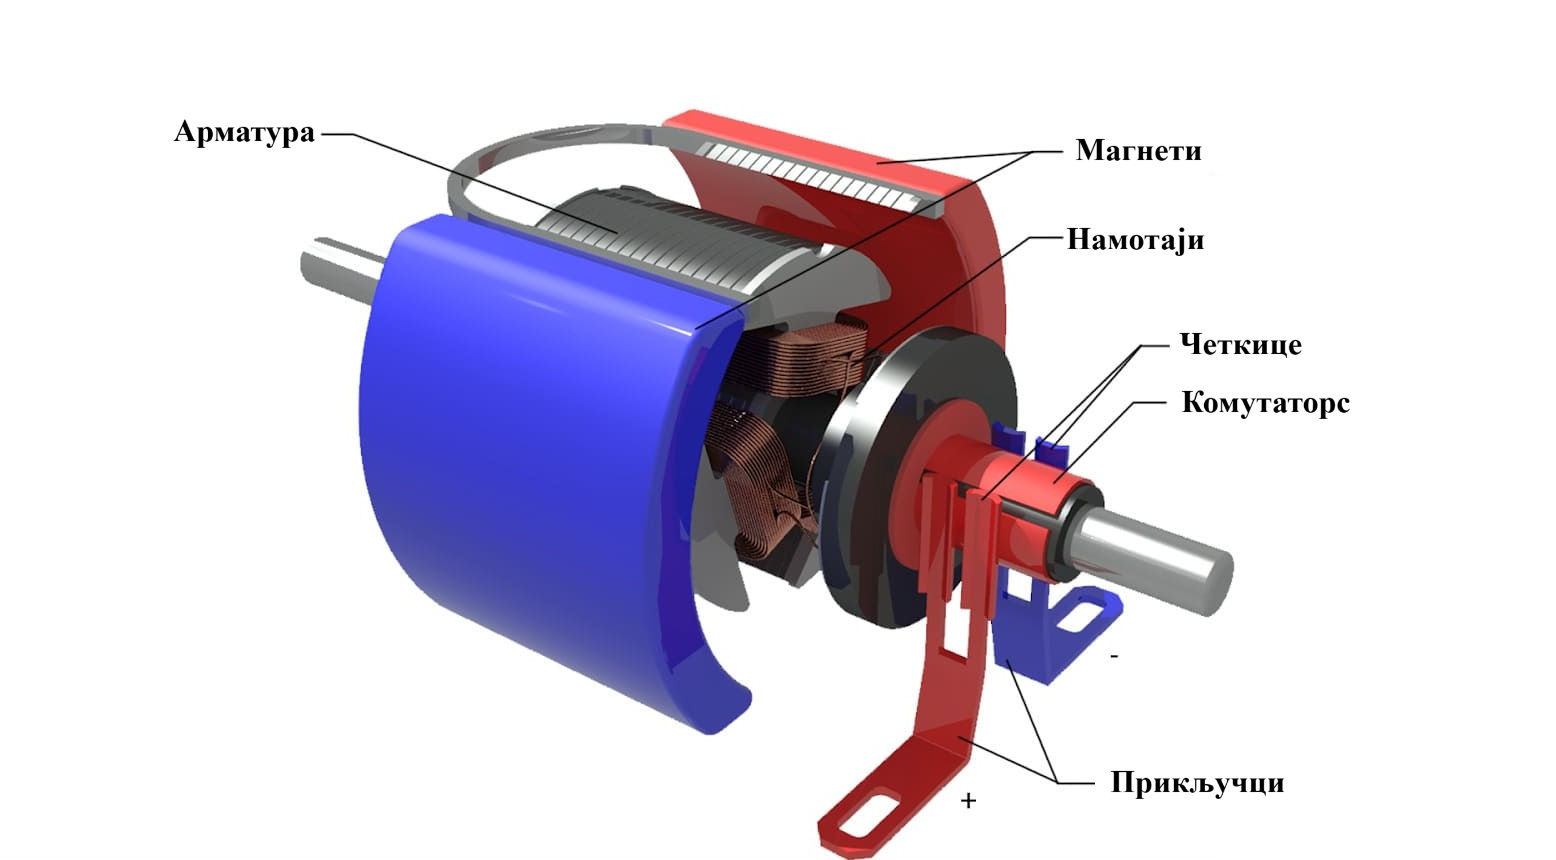
\includegraphics[height=2in]{Images/MotorJednosmerneStruje.jpg }
\caption{Приказ конструкције мотора једносмерне струје са четкицама.\cite{dc_motor_slika}}
\label{fig:figure12}
\end{figure}

\subsection{Инкрементални енкодер}
Инкрементални енкодер служи за одређивање брзине и положаја предмета током обртног кретања. Индустрија електричних мотора у великој мери уграђује енкодере на један крај вратила како би кориснику омогућила компактно паковање и интеграцију са мотором.\ \\
\\
Инкрементални енкодер је сачињен од два главна дела. Први је диск који се махнички круто веже за вратило мотора. На диску постоје прорези који су равномерно распоређени. Углавном је број прореза једнак броју експонента броја два (нпр. 512, 1024, 4096...) ради лакшег програмског манипулисања приликом обраде сигнала. Други део инкременталног енкодера је штампана плочица која на себи садржи фото предајник и фото пријемник. Како се енкодерски диск обрће, размак између прореза наизменично прекида светло између предајника и пријемника. Пријемник светла је реализован као прекидач и проводи струју само када има светла. Овим принципом се добијају импулси који се даље спроводе до микроконтролера.\\
Новији инкрементални енкодери углавном на диску имају две групе прореза које су смакнуте једна у односу на другу. На овај начин је резолуција мерења енкодера дупло већа, и притом је могуће добити информацију о смеру обртања енкодерског диска. Ова два сигнала се углавном називају "А" и "В". Поред две групе прореза, инкрементални енкодери често имају још један, одвојен, додатни прорез који служи да сигнализира када се диск обрне за један цео круг. Шематски приказ принципа рада енкодера дат је на слици 13.\ \\
\\
Предност инкременталних енкодера је релативно ниска цена и чињеница да их је веома лако користит. Мана инкременталних енкодера је корак (инкремент) који ограничава прецизност мерења позиције и брзине.
\cite{encoder}

\begin{figure}[H]
\centering
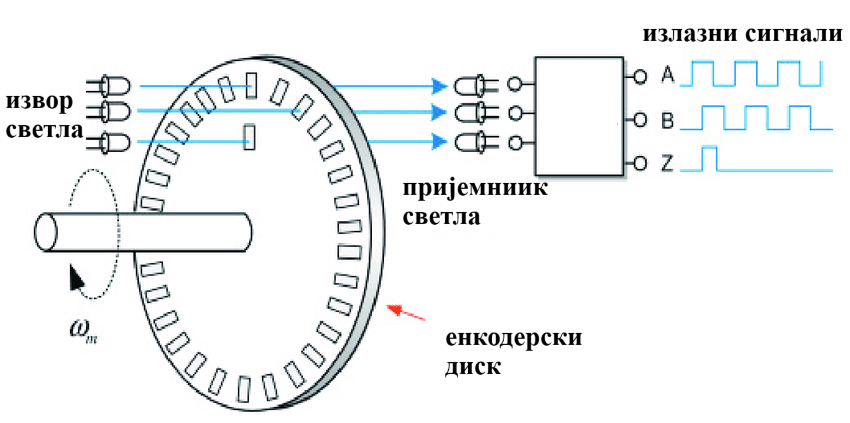
\includegraphics[height=2in]{Images/InkrementalniEnkoder.png }
\caption{Принцип рада енкодера.\cite{encoder}}
\label{fig:figure13}
\end{figure}

\subsection{\textit{CAN} комуникациони протокол}
\textit{CAN} комуникациони протокол је један од најкоришћенијих комуникационих протокола у индустрији. Због своје отпорности на шум највише се користи у аутомобилској индустрији. Због отпорности на шум, овај протокол преставља идеално решење у околини у којој је веома доминантно електромагнетно зрачење као што је непосредна брзина електричног мотора.
\textit{CAN} протокол подржава више надређених (енг. \textit{master}) и подређених (енг. \textit{slave}) уређаја. \\
Принцип отклањања шума на \textit{CAN} мрежи се заснива на логичком сабирању диференцијалних сигнала. Сигнал се кроз мрежу води кроз два проводника, \textit{CANH} и \textit{CANL}. Оба сигнала носе исту информацију али су симетрични (приказано на слици 14). Пријемник упоређује сигнале и ако им је напонски ниво различит приликом упоређивања, добијамо логичку нулу, а у колико је исти добијамо логичкu јединицу. У случају настанка шума, упоређивањем напонског нивоа добијамо исту разлику између напонских нивао оба сингла, као и да нема шума, чиме се проблем решава. Препоручљиво је да свака \textit{CAN} мрежа на својим крајевима између \textit{CANH} и \textit{CANL} линија има два отпорника од 120 \ohm како би се случајно пресликавање струје спречило. \\
\begin{figure}[H]
\centering
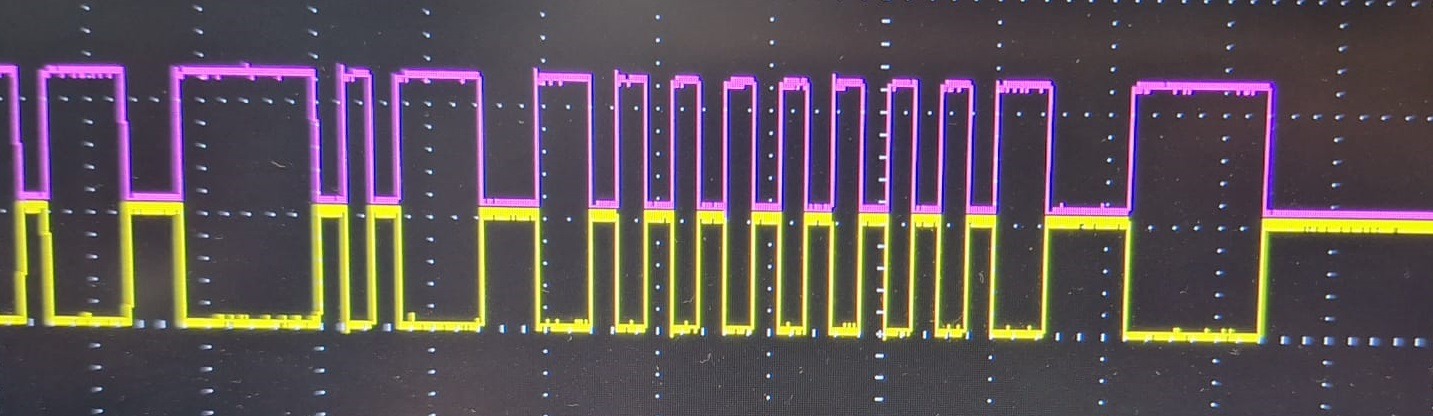
\includegraphics[height=1in]{Images/CAN_Osci.jpg }
\caption{\textit{CANH} и \textit{CANL} сигнали}
\label{fig:figure14}
\end{figure}
Формат сваке стандарне \textit{CAN} поруке је исти. Прва група бита у поруци се називају арбитрационо поље (енг. \textit{arbitatrion field}). На почетку се налази почетни бит (енг. \textit{start-of-frame (SOF)}) који поред означавања почетка поруке, служи и за усаглашавање свих уређаја на мрежи. Након почетног бита следи идентификатор (енг. \textit{identifier}) који је дужине једанаест бита, и носи информацију о томе које уређај шаље поруку. Последњи бит у арбитрационом пољу је \textit{remote transmission request (RTR)} бит који служи за зхтевање дозволе за слање поруке. Следће поље је контролно поље (енг. \textit{control field}). Први бит у контролном пољу је \textit{identifier extension (IDE)} који се користи само за случајеве проширене \textit{CAN} поруке, и он разликује проширену и стандардну поруку. Следећи је резервисани \textit{r0} бит. Последњи део овог сегмента поруке су \textit{data length code (DLC)}, који описују дужини информације која следи у поруци. Следећи елемнт поруке је сама информација (енг. \textit{data}) која се преноси и она може бити максимално осам бајтова, како би се омогућила што бржа трансмисија поруке. Следећи део поруке је \textit{cyclic redundancy check (CRC)}, представља софтверски вид заштите, а његова вредност је резултат формуле која сабира све битова, и на одређени начин их ставља у петнаестобитни низ. Предпоследњи члан поруке је acknowledgment (АСК) поље, које уређај који прима информацију користи да би потврдио пријем поруке. На крају се налази \textit{end-of-frame (EOF)} поље које се сасатоји од седам бита и означава крај једне \textit{CAN} поруке. Пример изгледа \textit{CAN} поруке дат је на слици 15.
\begin{figure}[H]
\centering
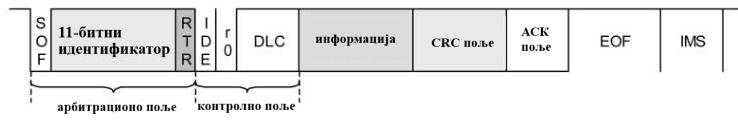
\includegraphics[height=1in]{Images/CAN_msg.png }
\caption{Структура \textit{CAN} поруке}
\label{fig:figure15}
\end{figure}

\subsection{\textit{UART} комуникациони протокол}
\textit{UART} комуникациони протокол је један од најстаријих дигиталних комуникационих протокола. Најчешће је коришћен за размену информација између рачунара и микроконтролера због релативно простог коришћења.\\
\textit{UART} комуникација се најчешће реализује у виду две топологије. Прва топологија се назива \textit{full duplex} и тада се сингали од, на пример рачунара ка микроконтролеру преносе кроз један проводник, док се сигнали од микроконтролера ка рачунару преносе кроз други. Поред \textit{full duplex} топологије постоји и \textit{half duplex} топологија где се сигнал у оба смера преноси кроз исти проводник и тада само један уређај може да шаље инфорације само у једном тренутку. Стандард је да свака линија, и за пријем и за слање, буде високог логичког нивоа док мрежа мирује.\\
Свака \textit{UART} порука је сачињена од истих сегмената. Први сегмент је стартни бит, и он означава почетак поруке спуштањем напона на линији на 0 V. Након стартног бита се смешта информација која се шаље, од најмање значајног бита (енг. \textit{least significant bit}), ка највише значајном биту (енг. \textit{most significant bit}). После битова који преносе информацју додаје се бит парности. Парност поруке се поставља на парну или непарну. У колико је парност подешена на паран број, бит парности ће бити постављен на нулу, и то означава да је број логичких јединица у поруци, заједно са битом парности паран број. У колико је парност подешена на непарно, бит парности ће бити постављен на логичку јединицу, чиме је број јединица у поруци заједно са битом парности непаран број. Бит парности се корсити за проверу да није дошло до грешке приликом слања, односно да су сви битови остали непромењени. На крају поруке се налази стоп бит, који увек има вредност логичке јединице и служи за враћање \textit{UART} линије у почетно стање. Приемр \textit{UART} поруке дат је на слици 16.

\subsection{Спуштач напона}
Спуштач напона (енг. \textit{Buck converter}) је врста претварача једносмерне струје. Као што им име каже, спуштачи напона служе да улазни напон смање на мању вредност, коју дају на излазу. Постоје две подела спуштача напона а то су синхрони и асинхрони спуштачи напона, приказано на слици 17. Оба типа раде на сличном принципу. Основне компоненте асинхроног спуштача напона су прекидачки елемент, диода, завојница и кондензатор. 
\begin{figure}[H]
\centering
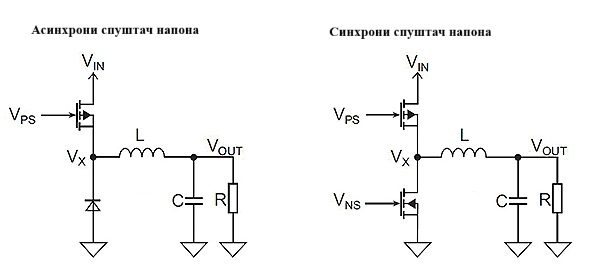
\includegraphics[height=2.5in]{Images/buck.jpg }
\caption{Електрична шема асинхроног и синхроног спуштача напона}
\label{fig:figure17}
\end{figure}
Основни принцип рада спуштача напона се заснива на узастопном прекидању прекидачког елемента, чиме струја наизменично пролази ка потрошачу. Излазни напон зависи од процента времена укључености прекидачког елемента, приказано на слици 17, у односу на циклус укључивања и искључивања, као што је показано у формули 1.\\
\begin{equation}
    U_{\text{излаз}} = \frac{T_{\text{укључено}}}{T_{\text{укључено}} + T_{\text{искључено}}} U_{\text{улаз}}
\end{equation}

Излатни напон прекидачког елемента се даље доводи на завојницу. Завојница служи да, док је прекидач укључен, складишти електричну енергију унутар себе, и да када се прекидач искључи, ту енергију пропусти даље ка потрошачу. \\
Диода се користи да затвори напонски круг када је прекидач исључен. Код синхроних спуштача напона, диода се мења прекидачким елементом, који проводи када је главни прекидачки елемент искључен.\\
Последња компонента спуштача напона је кондензатор, који служи да одржи стабилан излазни напон када је прекидачки елемент искључен и да варијације напона смањи на минимум.

\begin{figure}[H]
\centering
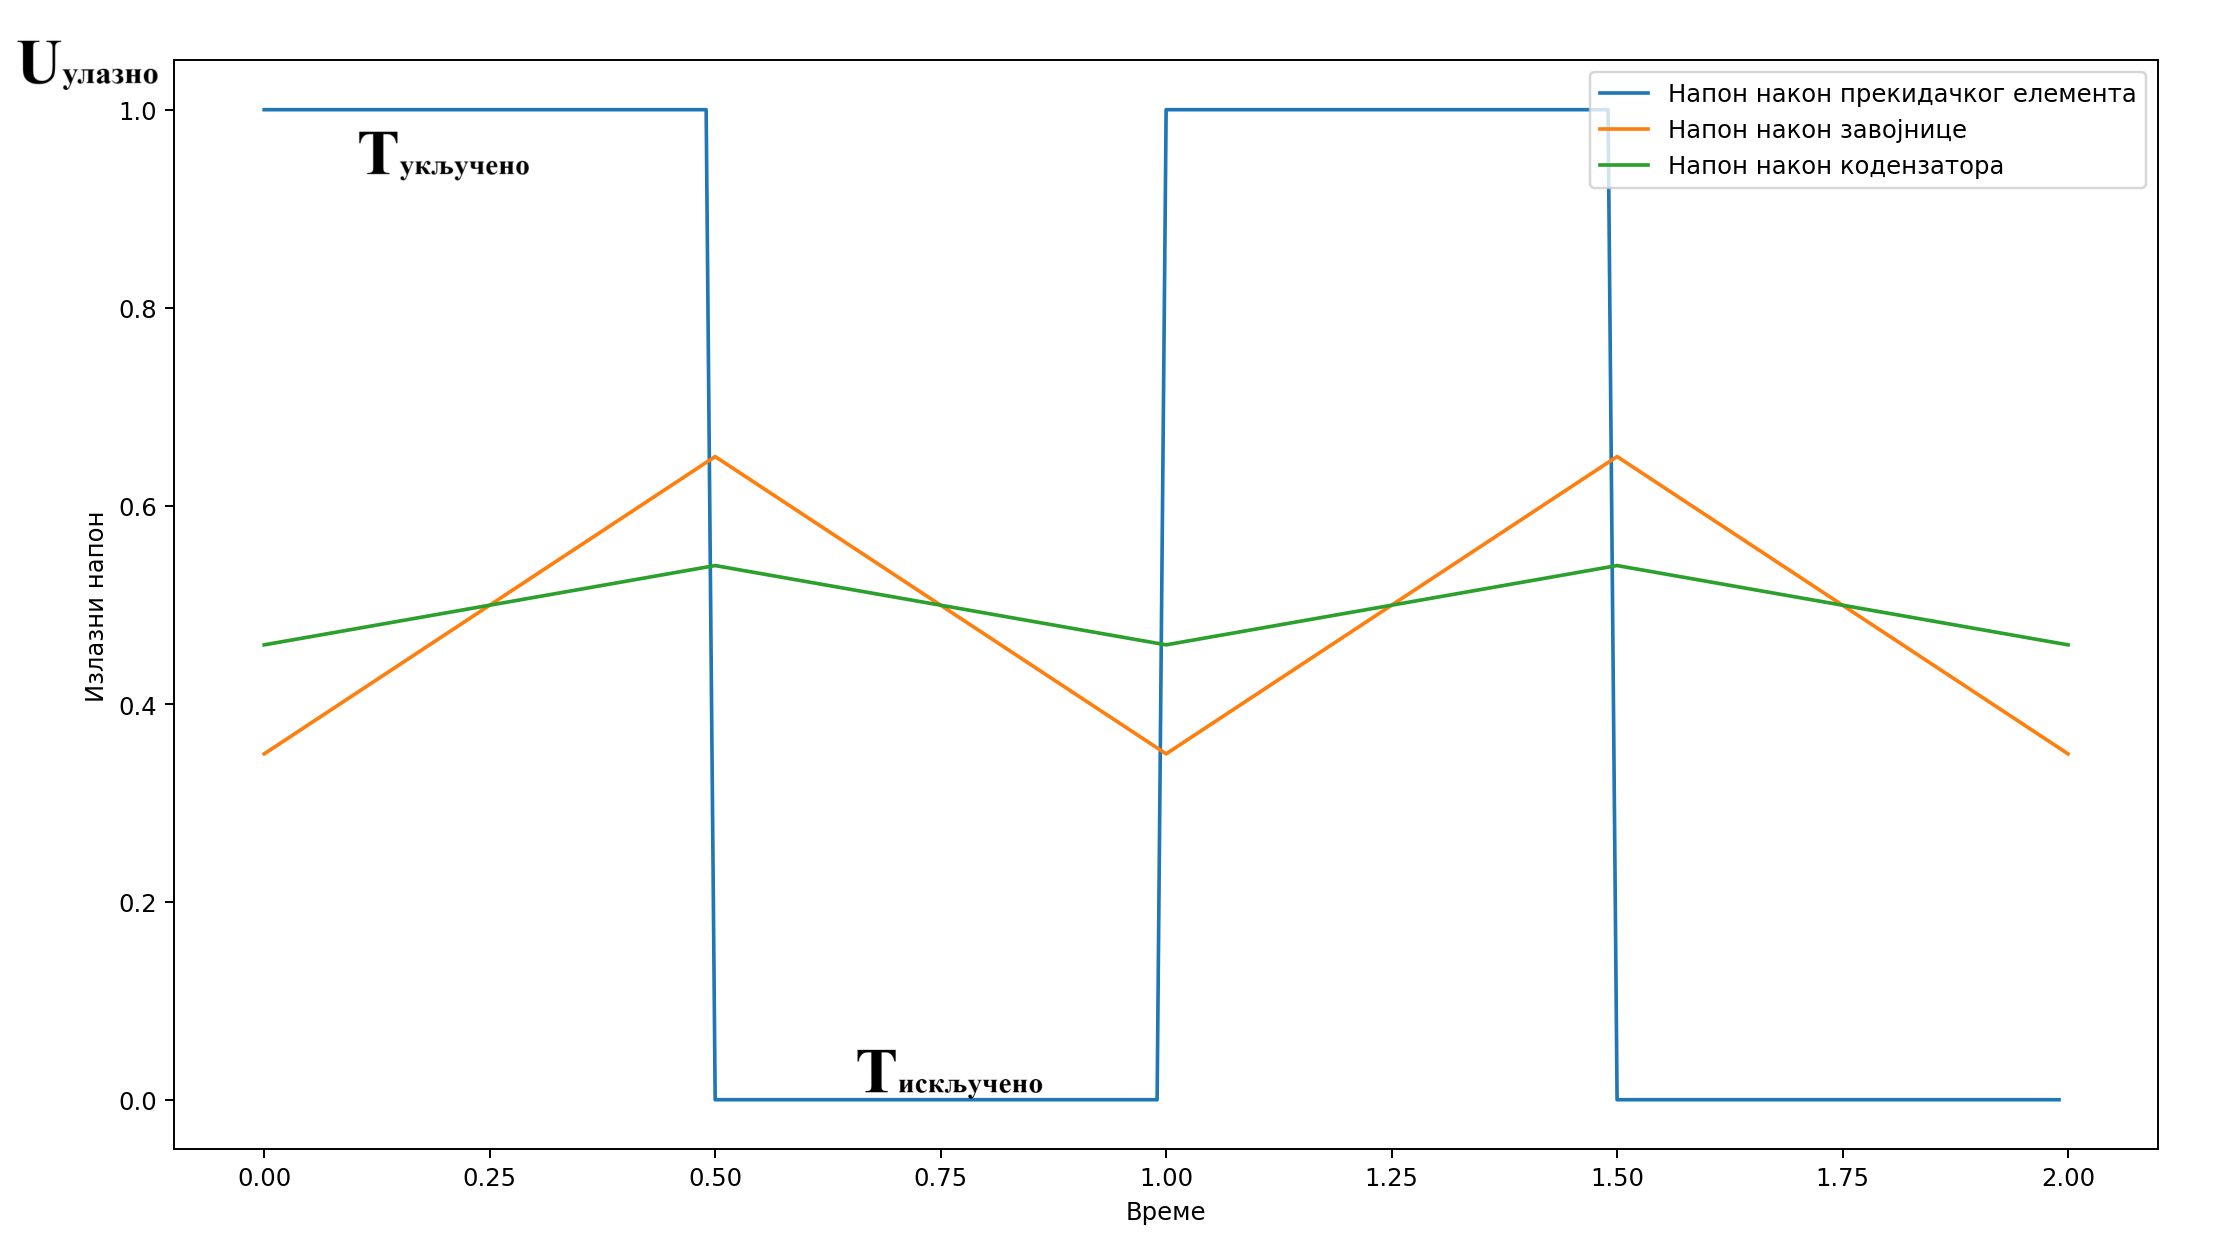
\includegraphics[height=2.3in]{Images/PWM.png }
\caption{Напон на илазу прекидачког елемента спуштача напона}
\label{fig:figure19}
\end{figure}
\clearpage

\subsection{Х мост}
Х мост (енг. \textit{H-bridge}) је електрично коло намењено за управљање брзином и смером обртања мотора једносмерне струје са четкицама. Коло је сачињено од четири прекидачка елемента. Сваки прикључак мотора је повезан са једним прекидачким елементом на високи напонски ниво, и са другим прекидачким елементом на ниски напонски ниво. Микроконтролер у зависности од смера обртања наизменично укључује и искључује два супротна прекидачка елемента, \textit{PWM} сигналом. Један прекидач спаја мотор са високим напонским нивоом, а други са нисаким напонским нивоом. и тиме се одређују смер и брзина обртања мотора. Шематски приказ повезивања Х моста и мотора је дат на слици 20.

\begin{figure}[H]
\centering
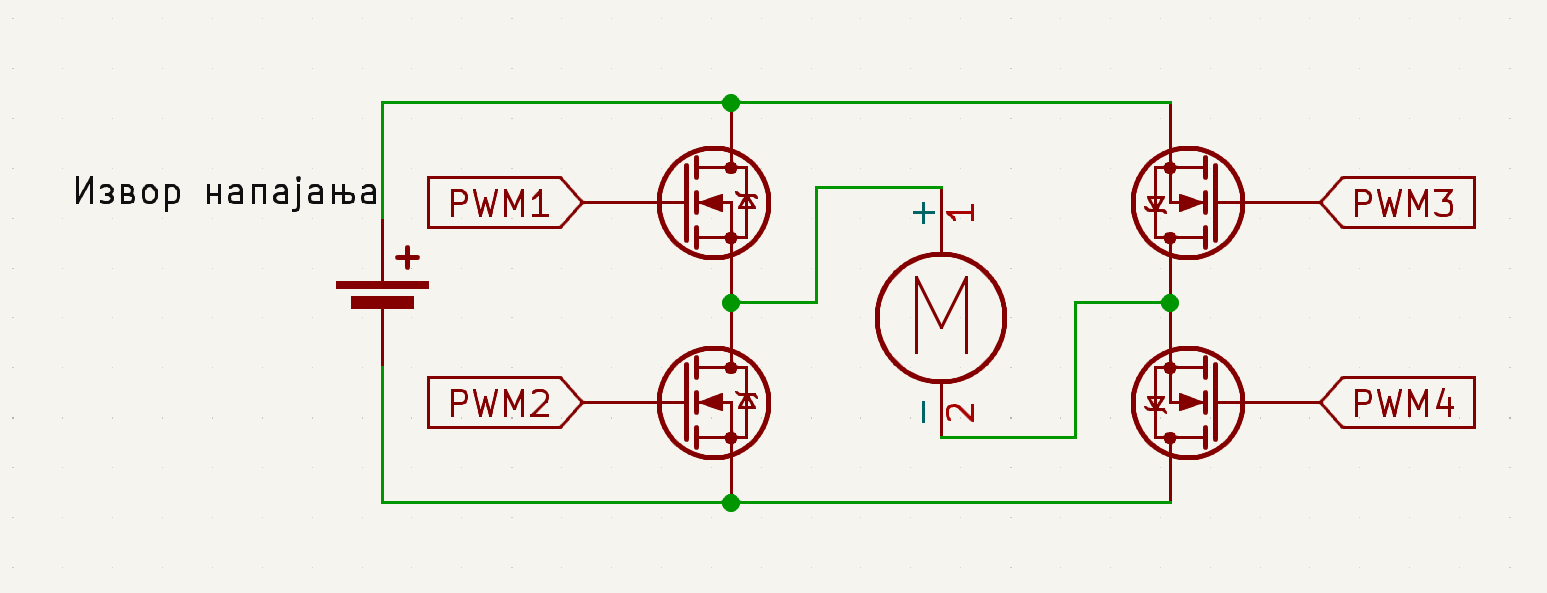
\includegraphics[height=2.3in]{Images/H_most.png }
\caption{Повезивање Х моста и мотора једносмерне струје са четкицама}
\label{fig:figure20}
\end{figure}
\clearpage

\printbibliography
\clearpage

\includepdf[pages = 2, scale = 0.85, angle = 90, pagecommand=\section{Прилог 1}]{HCU_PCB.pdf}
\includepdf[pages = 3-, scale = 0.85, angle = 90, pagecommand={}]{HCU_PCB.pdf}

\end{document}